% Provenance (never printed): see sources/outline_sources.md (Year 3:
% geomorphology, hillslope processes, river incision, landscape evolution).
% Brief: sources/book5/BRIEFS.md, ch. 18. Curves from
% figdata/bachelor-3/hillslope.py, stream_profile.py and varden_river.py.
% Exercise and problem values in the Book 5 scratch calculator calc/ch18.py.
% The upland west of the Varden Hills, its river, its tributaries, its
% uplift rate and its base-level fall are invented; the outlet elevation is
% the region model's river at the west edge of the map.
\chapter{Géomorphologie quantitative}\label{ch:b3:quantitative-geomorphology}

Une rivière qui traverse une chaîne en surrection présente une marche dans son profil longitudinal~: une cascade,
avec une gorge en aval et une vallée plus douce en amont. La marche ne reste pas
à l'endroit où elle s'est formée. Elle remonte vers l'amont, de quelques millimètres ou de quelques mètres
par an, et sa position est une horloge qui a commencé lorsque le \omterm{def:b3:quantitative-geomorphology:knickpoint}{niveau de base} de la rivière a été
abaissé. Lire cette horloge, ainsi que les taux inscrits dans la forme des collines
et des rivières, demande deux lois de conservation et deux lois de transport~: l'une pour le
sol qui se déplace lentement le long d'une pente, l'autre pour le substratum rocheux qu'une rivière entaille.

\begin{recall}
L'altération, l'érosion, le dépôt, les formes du relief et l'équilibre entre
soulèvement et érosion figurent dans les manuels scolaires, de même que le rebond isostatique et les
vallées glaciaires en U. Le taux de dénudation, la contrainte de cisaillement au fond et le
paramètre de Shields figurent dans le volume de première année, dans son chapitre sur l'érosion et le transport~;
le modèle numérique de terrain dans son chapitre sur les cartes géologiques~; l'isostasie d'Airy
dans son chapitre sur l'isostasie et les anomalies de pesanteur. Les \omterm{def:b3:advanced-geochronology:cosmogenic}{nucléides cosmogéniques}
et les taux d'érosion qui en découlent figurent
au chapitre~\ref{ch:b3:advanced-geochronology}, la \omterm{def:b3:orogenic-wedges:thermochronology}{thermochronologie} et la
\omterm{def:b3:orogenic-wedges:age-elevation}{relation âge--altitude} au chapitre~\ref{ch:b3:orogenic-wedges}.
L'équation de diffusion figure dans les volumes de physique.
\end{recall}

\section{Versants}\label{sec:b3:quantitative-geomorphology:hillslopes}

Sur une colline couverte de sol, celui-ci descend la pente grain à grain~: les animaux fouisseurs
le projettent, les racines le soulèvent, le gel et l'humectation le gonflent, et chaque
perturbation permet à la pesanteur de le déplacer un peu. Moyenné sur des siècles, le
flux de sol est proportionnel à la pente.

\begin{definition}[Diffusion de versant]\label{def:b3:quantitative-geomorphology:diffusion}
La \emph{diffusion de versant}\index{diffusion de versant} est le transport lent
de sol vers le bas du versant, dont le flux volumique par unité de largeur de pente,
$\vec q$, est proportionnel au gradient de la hauteur de surface $z$~:
$\vec q = -\kappa\,\nabla z$. Le coefficient $\kappa$, en
\unit{m^2/an}, est la diffusivité de versant.
\end{definition}

\begin{theorem}[Diffusion des versants]\label{thm:b3:quantitative-geomorphology:diffusion}
Supposons que la roche soit soulevée à un taux $U$ par rapport aux chenaux qui bordent un
versant, que le sol et la roche aient la même masse volumique, et que le sol se déplace par
\omterm{def:b3:quantitative-geomorphology:diffusion}{diffusion de versant} avec $\kappa$ uniforme. Alors la hauteur de surface obéit à
\[
\frac{\partial z}{\partial t} = U + \kappa\,\nabla^2 z ,
\]
l'équation de diffusion avec terme source.
\end{theorem}

\begin{proof}
Prenons une petite aire $\delta S$ du versant. Son volume varie par soulèvement,
$U\,\delta S$ par unité de temps, et par le sol qui sort à travers ses
bords, $\oint \vec q\cdot\vec n\,\mathrm{d}\ell = (\nabla\cdot\vec q)\,\delta S$.
D'où $\partial z/\partial t = U - \nabla\cdot\vec q$~; avec $\vec q = -\kappa
\nabla z$ et $\kappa$ uniforme, $\nabla\cdot\vec q = -\kappa\nabla^2 z$.
\end{proof}

Une faille ou un littoral découpe un escarpement à un instant donné~; ensuite, l'escarpement ne fait plus que
diffuser. Partant d'une marche verticale de demi-hauteur $a$ posée sur une pente
régionale $b$, la solution en une dimension est
\[
z(x,t) = a\,\operatorname{erf}\!\left(\frac{x}{2\sqrt{\kappa t}}\right) + b\,x ,
\qquad
\left.\frac{\partial z}{\partial x}\right|_{x=0} = \frac{a}{\sqrt{\pi\kappa t}} + b .
\]
La forme ne dépend que du produit $\kappa t$~: un profil mesuré donne
$\kappa t$, et soit un âge indépendant donne $\kappa$, soit un $\kappa$ connu donne
l'âge, un \emph{âge morphologique}. Les escarpements des régions semi-arides
à sols granulaires et à végétation clairsemée donnent un $\kappa$ compris entre
$10^{-3}$ et \qty{e-2}{m^2/an}~; les montagnes côtières humides et densément
végétalisées atteignent environ \qty{5e-3}{m^2/an}.
% ledger: whipple04:scarp-erf, whipple04:scarp-kappa

\begin{omfigure}
\begin{tikzpicture}
\begin{groupplot}[group style={group size=2 by 1, horizontal sep=1.6cm},
  width=0.48\linewidth, height=0.36\linewidth, tick label style={font=\scriptsize},
  label style={font=\small}, legend style={font=\scriptsize, draw=none, fill=none}]
\nextgroupplot[xlabel={distance $x$ (m)}, ylabel={$z$ (m)}, xmin=-40, xmax=40,
  ymin=-5, ymax=5, legend pos=north west]
% computed in figdata/bachelor-3/hillslope.py
\addplot[black!50, densely dashed] table[x=x, y=z0] {figdata/out/bachelor-3-hillslope-scarp.dat};
\addplot[omDef, thick] table[x=x, y=z1] {figdata/out/bachelor-3-hillslope-scarp.dat};
\addplot[omProp, thick] table[x=x, y=z2] {figdata/out/bachelor-3-hillslope-scarp.dat};
\addplot[omThm, thick] table[x=x, y=z3] {figdata/out/bachelor-3-hillslope-scarp.dat};
\legend{initial, \qty{2}{ka}, \qty{10}{ka}, \qty{40}{ka}}
\nextgroupplot[xlabel={distance à la ligne de partage (m)}, ylabel={hauteur (m)},
  xmin=-150, xmax=150, ymin=0, ymax=200, xtick={-150,-75,0,75,150}]
\addplot[omMeth, thick] table[x=x, y=z1] {figdata/out/bachelor-3-hillslope-hill.dat};
\addplot[omDef, thick] table[x=x, y=z2] {figdata/out/bachelor-3-hillslope-hill.dat};
\addplot[omThm, thick] table[x=x, y=z3] {figdata/out/bachelor-3-hillslope-hill.dat};
\node[font=\scriptsize, anchor=north] at (axis cs:0,45) {0.0215};
\node[font=\scriptsize, anchor=north] at (axis cs:0,94) {0.043};
\node[font=\scriptsize, anchor=north] at (axis cs:0,184) {\qty{0.086}{mm/an}};
\end{groupplot}
\end{tikzpicture}

\par\smallskip{\small À gauche, un escarpement de \qty{5}{m} de rejet sur une pente de
0.05, qui diffuse avec $\kappa = \qty{5e-3}{m^2/an}$~: la marche initiale
(en tirets) et les profils après 2, 10 et \qty{40}{ka}. À droite, des
collines à l'\omterm{def:b3:quantitative-geomorphology:steady-profile}{état stationnaire} de demi-largeur \qty{150}{m} avec le même $\kappa$ (hauteur au-dessus des
chenaux), s'abaissant à
0.0215, 0.043 et \qty{0.086}{mm/an}~: des paraboles dont le relief et la
courbure au sommet sont proportionnelles au taux d'érosion.}\label{fig:b3:quantitative-geomorphology:hillslope}
\end{omfigure}
% ledger: whipple04:scarp-kappa

Lorsqu'une colline a été soulevée et érodée suffisamment longtemps, sa forme cesse
de changer~: chaque point s'abaisse à la vitesse à laquelle la roche remonte.

\begin{proposition}[La courbure au sommet mesure le taux d'érosion]\label{prop:b3:quantitative-geomorphology:curvature}
Sur un versant à l'\omterm{def:b3:quantitative-geomorphology:steady-profile}{état stationnaire} sous l'effet de la \omterm{def:b3:quantitative-geomorphology:diffusion}{diffusion de versant}, le taux d'érosion
$E$, égal à $U$, vaut
\[
E = -\kappa\,\nabla^2 z .
\]
En une dimension, le profil est la parabole $z = z_0 - E x^2/(2\kappa)$,
avec un relief $E L^2/(2\kappa)$ entre la ligne de partage des eaux et les chenaux
situés à une distance $L$.
\end{proposition}

\begin{proof}
En posant $\partial z/\partial t = 0$ dans le théorème, on obtient $\kappa\nabla^2 z =
-U = -E$. En une dimension, deux intégrations avec $\mathrm{d}z/\mathrm{d}x =
0$ à la ligne de partage donnent la parabole, et sa valeur en $x = L$ donne le relief.
\end{proof}

La courbure, grandeur géométrique mesurée sur un modèle numérique de terrain, se lit donc
comme un taux dès que $\kappa$ est connu~: plus les sommets sont raides et arrondis
de façon marquée, plus le paysage s'érode vite. Le sol lui-même se forme à partir
de la roche sous-jacente, à un rythme qui dépend de la quantité de sol qui la recouvre déjà.

\begin{definition}[Fonction de production du sol]\label{def:b3:quantitative-geomorphology:soil-production}
La \emph{fonction de production du sol}\index{fonction de production du sol} donne
le taux $P$ auquel la roche en place se transforme en sol, en fonction de
l'épaisseur de sol $h$~; on la prend couramment égale à $P = P_0\,e^{-h/h_0}$, où
$P_0$ est le taux sur roche nue et $h_0$ une longueur d'une fraction de mètre.
\end{definition}

À l'\omterm{def:b3:quantitative-geomorphology:steady-profile}{état stationnaire}, l'interface sol-roche s'abaisse au rythme de la
surface, $P(h) = E$, de sorte que l'épaisseur de sol vaut $h = h_0 \ln(P_0/E)$~: une érosion
plus rapide donne un sol plus mince~; là où $E$ dépasse $P_0$, le sol est
arraché et la roche nue, limitée par l'altération, affleure. Les \omterm{def:b3:advanced-geochronology:cosmogenic}{taux de production} de sol les plus rapides
mesurés sont de l'ordre de \qty{0.5}{mm/an}.
% ledger: whipple04:soil

La diffusion linéaire ne tient pas sur les pentes raides. Lorsque le gradient approche
un seuil, les grains roulent et glissent par à-coups, et de petits glissements de terrain
arrachent le sol.

\begin{definition}[Pente critique du versant]\label{def:b3:quantitative-geomorphology:critical}
La \emph{pente critique du versant}\index{pente critique du versant}
$S_c$ est le gradient pour lequel le flux de sol croît sans limite~; dans une loi
de transport non linéaire largement utilisée, $q = \kappa S/[1 - (S/S_c)^2]$.
\end{definition}

Les pentes bien plus douces que $S_c$ se comportent comme dans la diffusion linéaire~; les pentes qui
s'érodent vite se raidissent vers $S_c$ et deviennent planes, leur gradient étant fixé par le
seuil plutôt que par le taux d'érosion.
% ledger: whipple04:nonlinear

\begin{inthefield}[Relevé d'un versant]
Une équipe qui étudie une crête recouverte de sol installe un scanner laser terrestre sur
un trépied, à quelques dizaines de mètres de la crête. Chaque balayage enregistre
des millions de points, c'est-à-dire la distance et la direction de la surface du sol, à travers les
trous de l'herbe et des arbustes~; les points de plusieurs stations sont fusionnés
en un seul nuage, recalé sur des cibles relevées au récepteur satellitaire,
et seuls les derniers retours sont conservés pour retirer la végétation. Le nuage de sol nu
est converti en modèle d'élévation à cellules décimétriques, lissé sur quelques
mètres, et son laplacien est calculé au niveau de la crête. L'équipe compare ensuite les
courbures au sommet de crêtes qui s'érodent à des taux mesurés avec des \omterm{def:b3:advanced-geochronology:cosmogenic}{nucléides
cosmogéniques}~: reportées l'une contre l'autre, les deux grandeurs donnent la diffusivité du
versant comme pente d'une droite, conformément à ce que prédit la proposition.
\end{inthefield}

\section{Incision fluviale}\label{sec:b3:quantitative-geomorphology:rivers}

Là où une rivière coule sur le substratum rocheux, elle se creuse en arrachant des blocs, par abrasion
sous sa charge de fond et par cavitation. Tous ces processus dépendent de la contrainte de
cisaillement que l'écoulement exerce sur son lit, ou de la puissance qu'il y dissipe, et tous deux
croissent avec le débit et la pente. Le débit croît avec l'aire drainée, si bien que l'aire
tient lieu de débit.

\begin{definition}[Loi de puissance fluviale]\label{def:b3:quantitative-geomorphology:stream-power}
La \emph{loi de puissance fluviale}\index{loi de puissance fluviale} donne le taux d'incision
verticale $E$ d'une rivière sur substratum rocheux~:
\[
E = K A^m S^n ,
\]
où $A$ est l'aire drainée en amont du point, $S$ la pente du
chenal, $m$ et $n$ des exposants positifs, et $K$ un coefficient d'érodabilité
qui regroupe la résistance de la roche, le climat et la largeur du chenal.
\end{definition}

Pour les processus qui dépendent de la contrainte de cisaillement ou de la puissance
spécifique de l'écoulement, $m/n$ est proche de 0.5. Une étude de chenaux de badlands creusés
dans une roche tendre pendant environ 20 ans a révélé des taux d'incision proportionnels à $A^{0.44}S^{0.68}$.
% ledger: whipple04:spim

\begin{definition}[Incision limitée par le détachement et incision limitée par le transport]\label{def:b3:quantitative-geomorphology:limited}
L'incision est \emph{limitée par le détachement}\index{incision limitée par le détachement}
lorsque la rivière peut évacuer plus de sédiments qu'elle n'en reçoit, de sorte que sa
vitesse d'abaissement est fixée par la rapidité avec laquelle elle détache le substratum de son lit~: la
\omterm{def:b3:quantitative-geomorphology:stream-power}{loi de puissance fluviale} s'applique. Elle est
\emph{limitée par le transport}\index{incision limitée par le transport} lorsque la rivière
transporte tous les sédiments qu'elle peut, de sorte que son lit ne s'abaisse qu'à l'endroit où
la capacité de transport augmente vers l'aval, au rythme fixé par la divergence
du flux sédimentaire.
\end{definition}

Une rivière \omterm{def:b3:quantitative-geomorphology:limited}{limitée par le transport} se comporte à peu près comme un versant~: le flux dépend
de la pente, et son profil évolue selon une équation de type diffusion qui arrondit
toute marche. Une rivière \omterm{def:b3:quantitative-geomorphology:limited}{limitée par le détachement} conserve une marche nette et la déplace,
comme le montre la section suivante. Les rivières de montagne au lit rocheux, couvert d'une
mince couche de graviers, sont en général plus proches du premier cas~; celles qui coulent sur
un alluvionnement épais relèvent plutôt du second.

\begin{omfigure}
\begin{tikzpicture}[x=0.55cm, y=0.55cm, font=\scriptsize,
  declare function={f(\x)=2.1+3.5*(1-(\x-0.5)/10)^2;
    tl(\x,\l)=f(\x)-1.1*exp(-(10.5-\x)/\l);}]
\begin{scope}
 \draw[->] (0,0) -- (11.5,0) node[below left] {distance vers l'aval};
\draw[->] (0,0) -- (0,6) node[above right] {$z$};
\draw[black!50, densely dashed] plot[domain=0.5:10.5, samples=40] (\x,{f(\x)});
\draw[omDef, thick] plot[domain=0.5:6.5, samples=30] (\x,{f(\x)}) -- plot[domain=6.5:10.5, samples=20] (\x,{f(\x)-1.1});
\draw[omThm, thick] plot[domain=0.5:3.5, samples=20] (\x,{f(\x)}) -- plot[domain=3.5:10.5, samples=30] (\x,{f(\x)-1.1});
\draw[->, black!70] (6.3,4.1) -- (3.8,4.75);
 \node[anchor=west, align=left] at (5.6,5.3) {limité par le détachement~:\\ la marche remonte vers l'amont};
\node at (5.5,-0.7) {(a)};
\end{scope}
\begin{scope}[xshift=7.2cm]
 \draw[->] (0,0) -- (11.5,0) node[below left] {distance vers l'aval};
\draw[->] (0,0) -- (0,6) node[above right] {$z$};
\draw[black!50, densely dashed] plot[domain=0.5:10.5, samples=40] (\x,{f(\x)});
\draw[omDef, thick] plot[domain=0.5:10.5, samples=40] (\x,{tl(\x,1.2)});
\draw[omThm, thick] plot[domain=0.5:10.5, samples=40] (\x,{tl(\x,3.5)});
 \node[anchor=west, align=left] at (5.0,5.3) {limité par le transport~:\\ l'abaissement diffuse vers l'amont};
\node at (5.5,-0.7) {(b)};
\end{scope}
\end{tikzpicture}

\par\smallskip{\small La réponse d'une rivière à un abaissement de son \omterm{def:b3:quantitative-geomorphology:knickpoint}{niveau de base}
(tirets~: le profil avant l'abaissement~; bleu, puis rouge~: deux instants ultérieurs),
schématique. (a) Une rivière \omterm{def:b3:quantitative-geomorphology:limited}{limitée par le détachement} conserve un \omterm{def:b3:quantitative-geomorphology:knickpoint}{knickpoint} marqué qui
migre vers l'amont~; en dessous, le profil garde son ancienne forme, abaissée. (b) Une
rivière abaisse progressivement tout son profil, surtout près
de l'exutoire.}\label{fig:b3:quantitative-geomorphology:regimes}
\end{omfigure}

Si les roches s'élèvent à un taux uniforme $U$ par rapport à l'exutoire de la rivière, et que $K$,
$m$, $n$ sont uniformes, la rivière évolue selon $\partial z/\partial t = U - K A^m
S^n$.

\begin{definition}[Profil de rivière en état stationnaire]\label{def:b3:quantitative-geomorphology:steady-profile}
Un profil de rivière est en \emph{état stationnaire}\index{état stationnaire}
lorsque son altitude ne change plus dans le temps~: en chaque point, l'incision
compense le soulèvement des roches par rapport à l'exutoire.
\end{definition}

\begin{theorem}[Profil en état stationnaire sous la loi de puissance fluviale]\label{thm:b3:quantitative-geomorphology:steady}
Si $U$, $K$, $m$ et $n$ sont uniformes, une rivière \omterm{def:b3:quantitative-geomorphology:limited}{limitée par le détachement}
en \omterm{def:b3:quantitative-geomorphology:steady-profile}{état stationnaire} possède le gradient
\[
S = \left(\frac{U}{K}\right)^{1/n} A^{-m/n} .
\]
\end{theorem}

\begin{proof}
À l'\omterm{def:b3:quantitative-geomorphology:steady-profile}{état stationnaire} $\partial z/\partial t = 0$, donc $K A^m S^n = U$, d'où $S^n
= (U/K)A^{-m}$~; en prenant la racine $n$-ième, on obtient le résultat.
\end{proof}

\begin{omfigure}
\begin{tikzpicture}
\begin{groupplot}[group style={group size=2 by 1, horizontal sep=1.7cm},
  width=0.48\linewidth, height=0.33\linewidth, tick label style={font=\scriptsize},
  label style={font=\small}]
\nextgroupplot[xlabel={distance à la ligne de partage des eaux (km)}, ylabel={$z$ (m)},
  xmin=0, xmax=12, ymin=150, ymax=420]
% computed in figdata/bachelor-3/stream_profile.py
\addplot[omDef, thick] table[x=d, y=z] {figdata/out/bachelor-3-stream_profile-steady.dat};
\nextgroupplot[xmode=log, ymode=log, xlabel={aire drainée $A$ (\unit{km^2})},
  ylabel={pente $S$}, xmin=0.1, xmax=100, ymin=0.003, ymax=0.2]
\addplot[omDef, thick] table[x=A, y=S] {figdata/out/bachelor-3-stream_profile-steady.dat};
\addplot[only marks, mark=*, mark size=1.4pt, omThm] table[x=A, y=S] {figdata/out/bachelor-3-stream_profile-sa.dat};
\addplot[omThm, densely dashed] table[x=A, y=S] {figdata/out/bachelor-3-stream_profile-fit.dat};
\end{groupplot}
\end{tikzpicture}

\par\smallskip{\small Le profil en \omterm{def:b3:quantitative-geomorphology:steady-profile}{état stationnaire} de la rivière fictive des hautes terres
à l'ouest des Varden Hills ($U = \qty{0.043}{mm/an}$, $K =
\qty{e-6}{an^{-1}}$, $m = 0.5$, $n = 1$), depuis sa tête de chenal jusqu'à
l'exutoire, à \qty{170}{m}. À droite, la pente en fonction de l'aire~: le modèle (ligne
bleue) et douze pentes mesurées sur des tronçons de \qty{200}{m} avec une
dispersion d'environ \qty{10}{\percent} (points rouges), dont la droite des moindres carrés
(tirets) a une pente de $-0.47$.}\label{fig:b3:quantitative-geomorphology:profile}
\end{omfigure}

La pente décroît en puissance de l'aire~: le profil est concave vers le haut. Les
rivières suivent une telle loi en puissance même lorsque les hypothèses du théorème sont
douteuses, deux nombres suffisent donc à résumer un profil.
% ledger: whipple04:steepness

\begin{definition}[Indices de raideur et de concavité du chenal]\label{def:b3:quantitative-geomorphology:indices}
Lorsque la pente d'une rivière suit $S = k_s A^{-\theta}$, l'exposant
$\theta$ est l'\emph{indice de concavité}\index{indice de concavité} et le
coefficient $k_s$ est l'\emph{indice de raideur du chenal}\index{indice de raideur du chenal}.
Pour comparer les rivières, $\theta$ est fixé à une valeur de référence commune
$\theta_{\mathrm{ref}}$, et $k_{sn} = S A^{\theta_{\mathrm{ref}}}$ est la
raideur normalisée.
\end{definition}

D'après le théorème, $\theta = m/n$ et $k_s = (U/K)^{1/n}$~: à érodabilité
donnée, une rivière est plus raide là où les roches se soulèvent plus vite. Les cartes de raideur
d'une chaîne soulignent donc son soulèvement.


Les pentes sont les dérivées d'altitudes bruitées et sont très dispersées. Intégrer
le profil utilise plutôt les altitudes, qui sont mieux mesurées.

\begin{definition}[Analyse en chi]\label{def:b3:quantitative-geomorphology:chi}
L'\emph{analyse en chi}\index{analyse en chi} trace l'altitude des points
d'un réseau fluvial en fonction de la coordonnée
\[
\chi(x) = \int_{x_b}^{x} \left(\frac{A_0}{A(x')}\right)^{\theta}
\mathrm{d}x' ,
\]
où $x$ est la distance vers l'amont le long du chenal depuis un point de base
$x_b$, $A_0$ une aire de référence et $\theta$ l'\omterm{def:b3:quantitative-geomorphology:indices}{indice de concavité}~; $\chi$ a
la dimension d'une longueur.
\end{definition}

\begin{proposition}[La transformation en chi redresse un profil stationnaire]\label{prop:b3:quantitative-geomorphology:chi}
Sous les hypothèses du théorème de l'\omterm{def:b3:quantitative-geomorphology:steady-profile}{état stationnaire}, avec $\theta = m/n$,
chaque chenal d'un réseau drainant vers l'altitude de base $z_b$ vérifie
\[
z = z_b + \left(\frac{U}{K A_0^{m}}\right)^{1/n} \chi~:
\]
tous les chenaux se trouvent sur une même droite de pente $k_s A_0^{-\theta}$ dans
le plan $(\chi, z)$.
\end{proposition}

\begin{proof}
Le long d'un chenal, $\mathrm{d}z/\mathrm{d}x = S = k_s A^{-\theta} = k_s
A_0^{-\theta}(A_0/A)^{\theta}$. En intégrant depuis $x_b$, où $z = z_b$,
on obtient $z = z_b + k_s A_0^{-\theta}\chi$, et $k_s A_0^{-\theta} =
(U/K)^{1/n} A_0^{-m/n}$. Un affluent rejoint le tronc à une confluence
où il partage $z$ et $\chi$ avec le tronc, et obéit à la même relation en amont de ce point.
\end{proof}

Un chenal qui s'écarte de la droite n'est pas en \omterm{def:b3:quantitative-geomorphology:steady-profile}{état stationnaire}, ou traverse
une roche d'érodabilité différente, ou a perdu ou capté de l'aire drainée~: un
affluent qui se place au-dessus de ses voisins à même $\chi$ est en train
de perdre de l'aire drainée au profit de ses voisins~; un affluent situé en dessous gagne de l'aire.

\section{Paysages transitoires}\label{sec:b3:quantitative-geomorphology:transient}

\begin{definition}[Niveau de base et knickpoint]\label{def:b3:quantitative-geomorphology:knickpoint}
Le \emph{niveau de base}\index{niveau de base} d'un cours d'eau est l'altitude de son
exutoire, en dessous de laquelle il ne peut inciser~: la mer, un lac ou le tronc
dans lequel il se jette. Un \emph{knickpoint}\index{knickpoint} est un endroit où la pente
du profil longitudinal d'un cours d'eau augmente brusquement, passant d'un tronçon
raidi à une chute d'eau.
\end{definition}

Un \omterm{def:b3:quantitative-geomorphology:knickpoint}{knickpoint} peut être fixe, lorsque le cours d'eau franchit un substrat plus dur ou un
escarpement de faille encore actif, ou mobile, lorsqu'il marque la tête de la
réaction du cours d'eau à une modification située en aval~: une baisse du \omterm{def:b3:quantitative-geomorphology:knickpoint}{niveau de base}, un
soulèvement plus rapide.
% ledger: whipple04:response

\begin{theorem}[Les knickpoints comme ondes cinématiques]\label{thm:b3:quantitative-geomorphology:kinematic}
Soit $n = 1$, avec $U$, $K$ et $m$ uniformes, et soit $x$ la distance
vers l'amont depuis l'exutoire. Alors $z$ vérifie
\[
\frac{\partial z}{\partial t} + K A^m \frac{\partial z}{\partial x} = U ,
\]
et toute particularité du profil, une marche comprise, se propage vers l'amont à la
célérité $c = K A^m$ en conservant sa hauteur. Un \omterm{def:b3:quantitative-geomorphology:knickpoint}{knickpoint} qui se forme
à l'exutoire à $t = 0$ atteint le point $x$ à l'instant
\[
t(x) = \int_0^x \frac{\mathrm{d}x'}{K A(x')^m} = \frac{\chi(x)}{K A_0^m},
\]
avec $\chi$ calculé pour $\theta = m$. Tous les \omterm{def:b3:quantitative-geomorphology:knickpoint}{knickpoints} nés dans un réseau
au même instant se trouvent donc au même $\chi$, et sur une même courbe de niveau.
\end{theorem}

\begin{proof}
Avec $x$ orienté vers l'amont, la pente vaut $S = \partial z/\partial x$, et
l'équation d'évolution $\partial z/\partial t = U - K A^m S$ est bien celle écrite.
Le long d'une courbe $\mathrm{d}x/\mathrm{d}t = K A(x)^m$, son membre de gauche
est la dérivée totale $\mathrm{d}z/\mathrm{d}t$, donc $z$ croît de $U$ par
unité de temps le long de chacune de ces courbes. Deux points de part et d'autre d'une marche,
portés par des courbes voisines, gagnent la même hauteur, si bien que la marche conserve
sa hauteur et se déplace avec les courbes. Le temps pour atteindre $x$ vaut
$\int \mathrm{d}x'/c$, soit $\chi(x)/(K A_0^m)$ par définition de
$\chi$ avec $\theta = m$. Dans le réseau, $\chi$ se mesure le long de chaque
ligne d'écoulement depuis le même exutoire~; des temps égaux signifient donc un même $\chi$, et, d'après
la proposition sur $\chi$, les tronçons situés sous les \omterm{def:b3:quantitative-geomorphology:knickpoint}{knickpoints}, déjà
ajustés au nouveau \omterm{def:b3:quantitative-geomorphology:knickpoint}{niveau de base}, les placent tous à la même altitude.
\end{proof}

La célérité croît avec l'aire drainée~: un \omterm{def:b3:quantitative-geomorphology:knickpoint}{knickpoint} progresse vite dans le
tronc et ralentit dans les têtes de bassin. Le temps qu'il met pour traverser tout le
réseau jusqu'aux têtes de chenal est le \emph{temps de réponse} du paysage,
de l'ordre du million d'années pour des taux de soulèvement typiques. Lorsque $n \ne 1$
la célérité dépend aussi de la pente, et une marche change de forme~: pour $n >
1$, sa face raide devance les tronçons qui l'entourent et reste nette~; pour $n <
1$, elle retarde et s'étale.

\begin{omfigure}
\begin{tikzpicture}
\begin{groupplot}[group style={group size=2 by 1, horizontal sep=1.5cm},
  width=0.5\linewidth, height=0.42\linewidth, tick label style={font=\scriptsize},
  label style={font=\small}, legend style={font=\scriptsize, draw=none, fill=none}]
\nextgroupplot[xlabel={distance à la ligne de partage des eaux (km)}, ylabel={$z$ (m)}, xmin=0, xmax=12.2,
  ymin=160, ymax=440, legend pos=north east]
% computed in figdata/bachelor-3/stream_profile.py
\addplot[black!50, densely dashed] table[x=d, y=z0] {figdata/out/bachelor-3-stream_profile-knick.dat};
\addplot[omMeth, thick] table[x=d, y=z1] {figdata/out/bachelor-3-stream_profile-knick.dat};
\addplot[omDef, thick] table[x=d, y=z2] {figdata/out/bachelor-3-stream_profile-knick.dat};
\addplot[omThm, thick] table[x=d, y=z3] {figdata/out/bachelor-3-stream_profile-knick.dat};
\legend{avant, \qty{300}{ka}, \qty{600}{ka}, \qty{900}{ka}}
\nextgroupplot[xlabel={$\chi$ (m)}, ylabel={$z$ (m)}, xmin=0, xmax=7500, ymin=160, ymax=520,
  scaled x ticks=false, xtick={0,2000,4000,6000}, xticklabels={0,2000,4000,6000},
  legend pos=north west]
% computed in figdata/bachelor-3/varden_river.py
\addplot[black!35, line width=2.2pt] table[x=chi, y=z] {figdata/out/bachelor-3-varden_river-trunk.dat};
\addplot[omMeth, only marks, mark=o, mark size=1.3pt, each nth point=8] table[x=chi, y=z] {figdata/out/bachelor-3-varden_river-trib1.dat};
\addplot[omDef, only marks, mark=square, mark size=1.2pt, each nth point=8] table[x=chi, y=z] {figdata/out/bachelor-3-varden_river-trib2.dat};
\addplot[omProp, only marks, mark=diamond, mark size=1.5pt, each nth point=8] table[x=chi, y=z] {figdata/out/bachelor-3-varden_river-trib3.dat};
\addplot[black, densely dashed, domain=0:7500, samples=2] {170 + 0.043*x};
\addplot[only marks, mark=triangle*, mark size=2.8pt, omThm] table[x=chi, y=zhi] {figdata/out/bachelor-3-varden_river-knicks.dat};
\legend{tronc, aff.~1, aff.~2, aff.~3, stationnaire}
\end{groupplot}
\end{tikzpicture}

\par\smallskip{\small À gauche, le cours d'eau de montagne après une baisse de \qty{25}{m} de
son \omterm{def:b3:quantitative-geomorphology:knickpoint}{niveau de base} ($n = 1$)~: le \omterm{def:b3:quantitative-geomorphology:knickpoint}{knickpoint}, une chute d'eau de hauteur constante,
atteint 1.7, 3.3 et \qty{4.6}{km} au-dessus de l'exutoire après 300, 600 et
\qty{900}{ka}~; en dessous, le cours d'eau garde l'ancienne forme, \qty{25}{m} plus bas.
À droite, diagramme en chi ($A_0 = \qty{1}{km^2}$, $\theta = 0.5$) du tronc et
de trois affluents à \qty{900}{ka}~: en dessous de $\chi = \qty{900}{m}$, chaque
chenal se trouve sur la droite de l'\omterm{def:b3:quantitative-geomorphology:steady-profile}{état stationnaire} passant par l'exutoire (tirets)~; au-dessus de cette valeur,
il se place sur l'ancienne droite, \qty{25}{m} plus haut. Les chutes d'eau du tronc et de
l'affluent 3 se situent au même $\chi$ (triangle rouge)~; les affluents 1 et 2 rejoignent
le tronc en amont de ce point et n'ont pas encore été
atteints.}\label{fig:b3:quantitative-geomorphology:knick}
\end{omfigure}

\begin{inthefield}[Une chute d'eau qui remonte vers l'amont]
\begin{minipage}[t]{0.40\linewidth}\vspace{0pt}
À Niagara, la rivière se jette dans une gorge qu'elle a elle-même creusée. Il y a environ
\num{12500} ans, les chutes se trouvaient au bord de l'escarpement du Niagara~;
depuis, à mesure que l'eau usait les roches de l'escarpement et que des blocs
se détachaient de la crête, celle-ci a reculé d'environ \qty{11}{km} vers l'amont,
soit en moyenne un mètre par an, et environ un dixième de cette valeur aujourd'hui.
L'érosion est plus lente lorsque la crête forme un long fer à cheval qui disperse
l'eau. La gorge est le chemin du \omterm{def:b3:quantitative-geomorphology:knickpoint}{knickpoint}.
\end{minipage}\hfill
\begin{minipage}[t]{0.56\linewidth}\vspace{0pt}
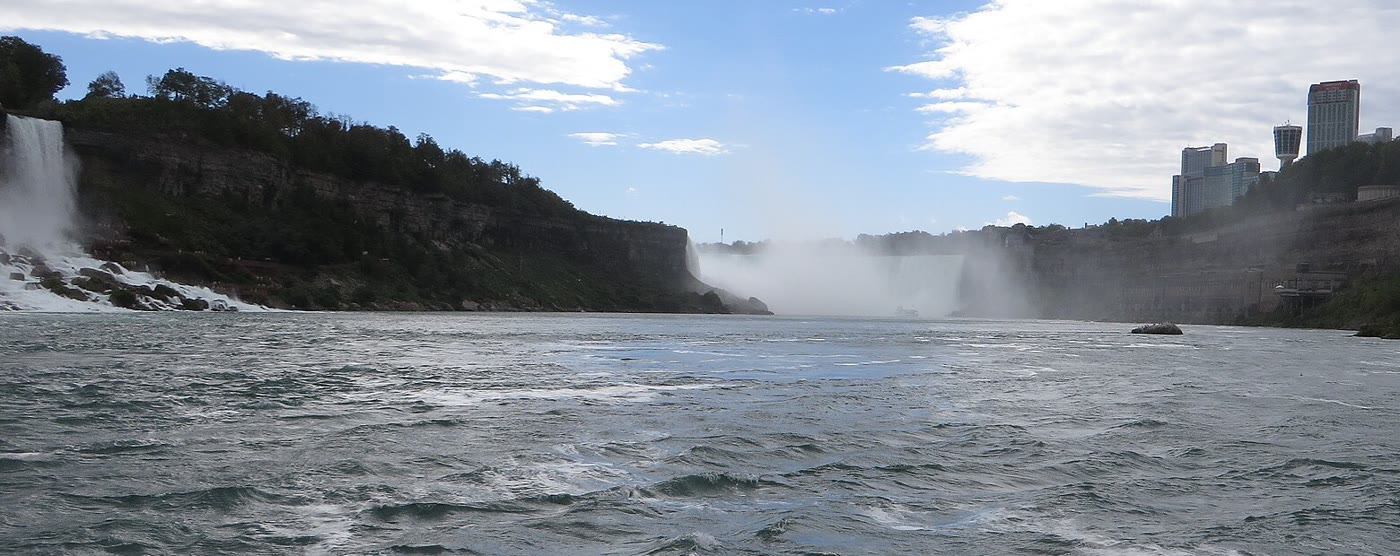
\includegraphics[width=\linewidth]{images/book5/b3-niagara-gorge.jpg}

{\scriptsize La gorge du Niagara, vue vers l'amont en direction des Horseshoe Falls dans
leur brume, les American Falls sur le bord gauche. Photo Ken Lund,
CC BY-SA 2.0 (recadrée).}
\end{minipage}
\end{inthefield}
% ledger: ijc18:niagara, photo:b3-niagara-gorge


\section{Érosion glaciaire}\label{sec:b3:quantitative-geomorphology:glacial}

Un glacier qui glisse sur son lit (glissement basal,
chapitre~\ref{ch:b3:glaciology}) l'érode par abrasion, les débris retenus dans la glace
raclant la roche, et par arrachement de blocs desserrés
par des fissures. Ces deux processus croissent avec la vitesse de glissement.

\begin{definition}[Loi d'érosion glaciaire]\label{def:b3:quantitative-geomorphology:glacial}
Une \emph{loi d'érosion glaciaire}\index{loi d'érosion glaciaire} donne le taux d'érosion
du lit d'un glacier sous la forme $E = K_G\,u_s^{\,l}$, où $u_s$ est la
vitesse de glissement, $K_G$ un coefficient et $l$ un exposant.
\end{definition}

Les modèles de paysage prennent généralement $l = 1$, avec des valeurs comprises entre 1 et 2 selon les études.
Une compilation portant sur 38 glaciers, dont les taux d'érosion s'étendent sur cinq ordres
de grandeur, a montré que l'érosion est corrélée à la vitesse de glissement, avec $l = 0.65$ et
$K_G = 10^{-4}$ pour $E$ en mètres par an~: l'érosion est la plus rapide sous les glaciers tempérés
alimentés par une neige abondante, qui glissent vite. La glace étant la plus épaisse
et la plus rapide le long de l'axe d'une vallée, le fond s'approfondit davantage que les
flancs, et la vallée prend sa forme en U.
% ledger: cook20:glacial

\begin{definition}[Scie circulaire glaciaire]\label{def:b3:quantitative-geomorphology:buzzsaw}
La \emph{scie circulaire glaciaire}\index{scie circulaire glaciaire} est la limite imposée à la
hauteur d'une chaîne de montagnes par les glaciers~: là où la roche s'élève au-dessus de l'altitude
à laquelle se forment les glaciers, ceux-ci l'érodent aussi vite qu'elle s'élève, quel que soit le
taux de soulèvement, de sorte que les sommets et l'altitude moyenne se regroupent près de cette altitude.
\end{definition}

\section{Tectonique et érosion}\label{sec:b3:quantitative-geomorphology:tectonics}

\begin{definition}[État stationnaire topographique]\label{def:b3:quantitative-geomorphology:steady-state}
Un paysage est dans un \emph{état stationnaire topographique}\index{etat stationnaire topographique@état stationnaire topographique}
lorsque son taux d'érosion égale partout le taux de soulèvement des roches, de sorte que
ses altitudes ne changent pas alors que la roche le traverse.
\end{definition}

Les taux mesurés sur des échelles de temps différentes permettent de tester cet état. Les \omterm{def:b3:advanced-geochronology:cosmogenic}{nucléides cosmogéniques}
contenus dans le sable des rivières donnent le taux d'érosion moyen d'un bassin pendant le temps
nécessaire à l'enlèvement d'une couche de l'ordre de la longueur d'atténuation de leur
production, soit environ \qty{55}{cm} de roche~; les \omterm{def:b3:orogenic-wedges:thermochronology}{thermochronomètres} et leurs \omterm{def:b3:orogenic-wedges:age-elevation}{relations âge--altitude} donnent
la vitesse d'exhumation sur plusieurs millions d'années. Lorsque les deux concordent entre eux
et avec le taux de soulèvement, le paysage est vraisemblablement dans un \omterm{def:b3:quantitative-geomorphology:steady-profile}{état stationnaire}~; lorsque
le taux à court terme est plus rapide dans le cours inférieur que dans les zones de source,
un \omterm{def:b3:quantitative-geomorphology:knickpoint}{knickpoint} est en train de migrer. Enlever de la roche décharge aussi la
lithosphère, qui se soulève en conséquence.
% ledger: zech04:exposure

\begin{definition}[Rebond isostatique d'érosion]\label{def:b3:quantitative-geomorphology:rebound}
Le \emph{rebond isostatique d'érosion}\index{rebond isostatique d'érosion} est
la remontée de la surface rocheuse d'une région en équilibre isostatique en
réponse à la masse enlevée par l'érosion.
\end{definition}

\begin{proposition}[Les sommets s'élèvent à mesure que les vallées s'approfondissent]\label{prop:b3:quantitative-geomorphology:rebound}
Dans l'isostasie d'Airy, avec une croûte de masse volumique $\rho_c$ reposant sur un manteau
de masse volumique $\rho_m$, l'enlèvement d'une épaisseur moyenne $\bar e$ de croûte sur une région élève
l'ensemble de la région de $(\rho_c/\rho_m)\,\bar e$. Si l'érosion se limite
aux vallées, les sommets non érodés remontent de cette quantité, tandis que la surface moyenne
ne s'abaisse que de $(1 - \rho_c/\rho_m)\,\bar e$.
\end{proposition}

\begin{proof}
La compensation exige que la masse de chaque colonne située au-dessus d'une profondeur fixe reste
la même. Enlever une épaisseur $\bar e$ de croûte, moyennée sur l'aire
de compensation, abaisse la masse par unité de surface de $\rho_c \bar e$~; la remplacer exige
que le manteau afflue en profondeur, soulevant la base de la
colonne, et tout ce qui la surmonte, de $\delta$ avec $\rho_m \delta = \rho_c \bar
e$. Un sommet qui n'a rien perdu s'élève de $\delta$~; la surface moyenne perd
$\bar e$ et gagne $\delta$.
\end{proof}

La masse volumique moyenne pondérée par l'épaisseur de la croûte du modèle de Terre de référence vaut
\qty{2.72}{g/cm^3} et celle du manteau situé sous son Moho \qty{3.38}{g/cm^3},
soit un rapport de 0.80~: pour chaque centaine de mètres de roche érodée, la surface moyenne ne perd que vingt mètres.
Une incision profonde d'un vieux plateau peut ainsi en élever les sommets
alors même que le plateau s'use.
% ledger: prem:crust-mantle-ratio

\begin{omfigure}
\begin{tikzpicture}[x=0.6cm, y=0.6cm, font=\scriptsize]
\begin{scope}
\fill[omDef!12] (0,0) rectangle (8,4);
\draw[thick] (0,4) -- (8,4);
\draw[densely dashed] (0,0) -- (8,0);
\node[anchor=north] at (4,-0.1) {base de la croûte};
\node at (4,2) {croûte $\rho_c$};
\node at (4,-1.2) {manteau $\rho_m$};
\node[anchor=south] at (4,4.1) {avant};
\end{scope}
\begin{scope}[xshift=6.2cm]
\fill[omDef!12] (0,0.8) -- (0,4.8) -- (1.4,4.8) -- (2.0,2.4) -- (2.6,4.8) -- (5.4,4.8) -- (6.0,2.4) -- (6.6,4.8) -- (8,4.8) -- (8,0.8) -- cycle;
\draw[thick] (0,4.8) -- (1.4,4.8) -- (2.0,2.4) -- (2.6,4.8) -- (5.4,4.8) -- (6.0,2.4) -- (6.6,4.8) -- (8,4.8);
\draw[black!50, densely dashed] (0,4) -- (8,4);
\draw[densely dashed] (0,0.8) -- (8,0.8);
\draw[densely dashed, black!40] (0,0) -- (8,0);
\draw[<->, omThm] (8.3,4.05) -- (8.3,4.75) node[midway, right] {$\delta$};
\draw[<->, omThm] (8.3,0.05) -- (8.3,0.75) node[midway, right] {$\delta$};
\node[anchor=west, font=\scriptsize] at (8.1,2.4) {$\delta = (\rho_c/\rho_m)\,\bar e$};
\node[anchor=south] at (4,5.0) {après incision des vallées};
\node[anchor=north] at (2.0,2.3) {vallée};
\end{scope}
\end{tikzpicture}

\par\smallskip{\small \omterm{def:b3:quantitative-geomorphology:rebound}{Rebond isostatique d'érosion}, schéma. Le creusement des
vallées retire une épaisseur moyenne $\bar e$ de croûte~; la colonne se soulève de
$\delta = (\rho_c/\rho_m)\bar e$ à sa base et à ses sommets non entaillés
(la ligne grise en pointillés figure l'ancienne surface).}\label{fig:b3:quantitative-geomorphology:rebound}
\end{omfigure}

\section{Exercices}

\begin{exercise}[$\star$]\label{exo:b3:quantitative-geomorphology:1}
Un escarpement de rivage de rejet \qty{4}{m} ($a = \qty{2}{m}$) se trouve
sur une pente lointaine de 0.04, et son gradient maximal vaut désormais 0.30. Calculer
$\kappa t$, puis l'âge de l'escarpement avec $\kappa = \qty{5e-3}{m^2/an}$.
\end{exercise}
% ledger: whipple04:scarp-erf, whipple04:scarp-kappa

\begin{exercise}[$\star$]\label{exo:b3:quantitative-geomorphology:2}
Un levé lidar donne une courbure de sommet de \qty{-0.012}{m^{-1}} sur une crête
de diffusivité \qty{4e-3}{m^2/an}. Calculer son taux d'érosion en
\unit{mm/an}, ainsi que le relief entre sa crête et les chenaux situés
à \qty{80}{m} de distance, en supposant un \omterm{def:b3:quantitative-geomorphology:steady-profile}{état stationnaire}.
\end{exercise}

\begin{exercise}[$\star$]\label{exo:b3:quantitative-geomorphology:3}
Avec $m = 0.5$, $n = 1$ et $K = \qty{2e-6}{an^{-1}}$, calculer le taux
d'incision d'une rivière drainant \qty{25}{km^2} sur une pente de 0.01.
Quelles sont les unités de $K$ pour $m$ et $n$ quelconques~?
\end{exercise}

\begin{exercise}[$\star$]\label{exo:b3:quantitative-geomorphology:4}
Trois rivières présentent des \omterm{def:b3:quantitative-geomorphology:knickpoint}{knickpoints}~: (a) là où un banc de grès recoupe une vallée
creusée dans des schistes~; (b) là où une rivière franchit une faille normale active,
du mur vers le toit~; (c) dans chacune des rivières d'un bassin, toutes à peu près
à la même altitude, à quelques kilomètres en amont d'une côte qui s'est soulevée
lors d'un séisme. Lesquelles sont fixes et lesquelles vont migrer~?
\end{exercise}

\begin{exercise}[$\star\star$]\label{exo:b3:quantitative-geomorphology:5}
Pour $m = 1$ et $n = 2$, calculer $\theta$ et la pente stationnaire là où $A =
\qty{10}{km^2}$, avec $U = \qty{0.1}{mm/an}$ et $K = 10^{-9}$ en mètres et
années.
De quel facteur l'indice de raideur change-t-il si $U$ double~? Comparer avec $n =
1$.
\end{exercise}

\begin{exercise}[$\star\star$]\label{exo:b3:quantitative-geomorphology:6}
L'aire drainée d'une rivière croît avec la distance $d$ à sa ligne de partage des eaux selon $A =
c\,d^{h}$. Montrer que, mesurée vers l'amont depuis son exutoire en $d = L$,
\[
\chi(d) = \frac{A_0^{\theta}}{c^{\theta}}\,\frac{L^{p} - d^{p}}{p},
\qquad p = 1 - h\theta ,
\]
et la calculer pour $c = 2$ (SI), $h = 1.8$, $\theta = 0.45$, $A_0 =
\qty{1}{km^2}$, $L = \qty{20}{km}$ et $d = \qty{5}{km}$.
\end{exercise}

\begin{exercise}[$\star\star$]\label{exo:b3:quantitative-geomorphology:7}
Avec $n = 1$, $m = 0.5$ et $K = \qty{2e-6}{an^{-1}}$, calculer la
célérité d'un \omterm{def:b3:quantitative-geomorphology:knickpoint}{knickpoint} où $A = \qty{100}{km^2}$, en m/ka, et le temps
qu'il mettrait pour parcourir \qty{5}{km} à cette vitesse. Pourquoi
prend-il en réalité plus de temps~?
\end{exercise}

\begin{exercise}[$\star\star$]\label{exo:b3:quantitative-geomorphology:8}
Des vallées de \qty{600}{m} de profondeur, occupant en moyenne \qty{40}{\percent} de la
surface d'un plateau, y sont entaillées. Avec $\rho_c/\rho_m = 0.80$, calculer
l'épaisseur moyenne érodée, le soulèvement des sommets et la variation de
l'altitude moyenne.
\end{exercise}
% ledger: prem:crust-mantle-ratio

\begin{exercise}[$\star\star$]\label{exo:b3:quantitative-geomorphology:9}
Une \omterm{def:b3:quantitative-geomorphology:soil-production}{fonction de production du sol} admet $P_0 = \qty{0.3}{mm/an}$ et $h_0 =
\qty{0.5}{m}$. Calculer l'épaisseur de sol stationnaire pour une érosion de
\qty{0.05}{mm/an} et de \qty{0.2}{mm/an}. Que se passe-t-il à
\qty{0.4}{mm/an}~?
\end{exercise}

\begin{exercise}[$\star\star\star$]\label{exo:b3:quantitative-geomorphology:10}
Une colline en \omterm{def:b3:quantitative-geomorphology:steady-profile}{état stationnaire} s'érode à $E = \qty{0.1}{mm/an}$ avec $\kappa =
\qty{5e-3}{m^2/an}$ et la loi non linéaire de la pente critique, en prenant
$S_c = 1.2$ pour l'exercice. Montrer que le flux à une distance $x$ de la
ligne de partage des eaux vaut $E x$, résoudre pour le gradient, et le calculer à 20, 50, 100 et
\qty{200}{m}. Comparer avec la diffusion linéaire et décrire la forme de la
colline.
\end{exercise}

\begin{exercise}[$\star\star\star$]\label{exo:b3:quantitative-geomorphology:11}
Montrer que le temps de réponse d'un réseau hydrographique à une variation
survenant à son exutoire vaut, pour $n = 1$, $\chi_h/(K A_0^m)$, où $\chi_h$ est la plus grande valeur
de $\chi$ en tête de chenal. Le calculer pour la rivière de plateau des figures
($A_0 = \qty{1}{km^2}$, $m = 0.5$, $K = \qty{e-6}{an^{-1}}$), d'abord pour son
tronc seul, dont la tête est à $\chi = \qty{5464}{m}$, puis pour le réseau,
dont la tête la plus haute, sur l'affluent 1, est à $\chi = \qty{7237}{m}$.
\end{exercise}

\begin{exercise}[$\star\star\star$]\label{exo:b3:quantitative-geomorphology:12}
Dans un réseau où $n = 1$ et $U$ est uniforme, un affluent s'écoule sur une roche deux
fois plus érodable que le reste ($2K$) au-dessus de sa confluence, en $\chi_j$. Montrer que
sa ligne stationnaire dans le plan $(\chi, z)$ a une pente égale à la moitié de celle du
tronc au-dessus de $\chi_j$, et qu'un \omterm{def:b3:quantitative-geomorphology:knickpoint}{knickpoint} né à l'exutoire atteint, au moment où
le \omterm{def:b3:quantitative-geomorphology:knickpoint}{knickpoint} du tronc se trouve en $\chi_k > \chi_j$, le point
de $\chi = \chi_j + 2(\chi_k - \chi_j)$ de cet affluent.
\end{exercise}

\section{Problème~: la chute d'eau de la rivière de Varden}

\begin{problem}[{Problème du week-end --- le profil, la raideur et l'érodabilité
d'une rivière de plateau fictive, et l'âge de sa chute d'eau}]
\label{pb:b3:quantitative-geomorphology:1}
À l'ouest des collines de Varden, la rivière draine un plateau de schistes avant
d'entrer sur la carte par son bord ouest, à une altitude de \qty{170}{m}. En amont
de ce point, son exutoire, le tronc mesure \qty{12}{km} de long depuis sa ligne de partage des eaux,
avec une aire drainée $A = 4.5\,d^{1.7}$ (\unit{m^2}, $d$ en mètres à partir de la
ligne de partage des eaux) et une tête de chenal à $d = \qty{300}{m}$. Prendre comme taux de soulèvement des roches
le taux de dénudation du bassin de la rivière de Varden, obtenu à partir de ses
charges, dans le volume de première année, \qty{43}{m/Ma}. Poser $n = 1$ et l'aire de référence $A_0 = \qty{1}{km^2}$.
Une chute d'eau haute de \qty{25}{m} se trouve sur le tronc, à \qty{4.60}{km} en amont de
l'exutoire. Toutes les valeurs sont fictives.

\medskip\noindent\textbf{Partie I --- Le profil.}
\begin{enumerate}
\item Calculer l'aire drainée à l'exutoire et à la tête de chenal.
\item Pentes mesurées sur des tronçons de \qty{200}{m}, à l'écart de la
  chute d'eau~:

  \smallskip
  {\small\begin{tabular}{l*{6}{c}}
  $A$ (\unit{km^2}) & 0.388 & 0.587 & 0.888 & 1.345 & 2.036 & 3.082 \\
  $S$ & 0.06641 & 0.05026 & 0.04888 & 0.03322 & 0.03688 & 0.02688 \\[2pt]
  $A$ (\unit{km^2}) & 4.665 & 7.061 & 10.69 & 16.18 & 24.49 & 37.08 \\
  $S$ & 0.01921 & 0.01713 & 0.01545 & 0.01419 & 0.007922 & 0.007855
  \end{tabular}}

  \smallskip
  Estimer l'\omterm{def:b3:quantitative-geomorphology:indices}{indice de concavité} à partir du premier et du dernier point.
\item La pente des moindres carrés de $\log S$ en fonction de $\log A$ vaut $-0.466$.
  Est-elle compatible avec $\theta = 0.5$~?
\item Avec $\theta_{\mathrm{ref}} = 0.5$, calculer $k_{sn} = S A^{0.5}$ ($A$ en
  \unit{m^2}) pour le premier et le dernier point, et dire ce que
  représente la moyenne géométrique des douze valeurs, \qty{45.1}{m}.
\item Pourquoi les pentes sont-elles beaucoup plus dispersées que les altitudes~?
\item En utilisant la formule de l'exercice sur le chi, calculer $\chi$ à $d =
  \qty{9.00}{km}$, en un point situé sous la chute d'eau.
\end{enumerate}

\medskip\noindent\textbf{Partie II --- Raideur et érodabilité.}
\begin{enumerate}[resume]
\item La rivière se trouve à \qty{193.4}{m} pour $d = \qty{9.00}{km}$. Calculer la
  pente de la courbe en chi sous la chute d'eau et la raideur $k_{sn}$.
\item Quelle estimation de $k_{sn}$ retenir, celle-ci ou celle issue de la
  méthode pente--aire, et pourquoi~?
\item En supposant un \omterm{def:b3:quantitative-geomorphology:steady-profile}{état stationnaire} sous la chute d'eau, calculer $K$ à partir du
  taux de soulèvement.
\item Vérifier que le taux d'incision à l'exutoire, dont la pente vaut
  0.00691, est égal au taux de soulèvement.
\item Calculer la célérité d'un \omterm{def:b3:quantitative-geomorphology:knickpoint}{knickpoint} à l'exutoire et à la
  chute d'eau, en m/ka.
\item Calculer l'altitude de la tête de chenal sur le profil stationnaire, et
  le dénivelé du tronc.
\end{enumerate}

\medskip\noindent\textbf{Partie III --- La chute d'eau.}
\begin{enumerate}[resume]
\item Pourquoi, avec $n = 1$, la chute d'eau a-t-elle conservé la hauteur de la
  baisse du \omterm{def:b3:quantitative-geomorphology:knickpoint}{niveau de base}~?
\item Calculer $\chi$ à la chute d'eau.
\item Calculer le temps mis par le \omterm{def:b3:quantitative-geomorphology:knickpoint}{knickpoint} pour aller de l'exutoire à sa
  position actuelle.
\item Où se trouvera-t-il d'ici \qty{300}{ka}~?
\item L'affluent~3 rejoint le tronc à \qty{2.5}{km} en amont de l'exutoire~; il
  mesure \qty{5}{km} de long, avec $A = 1.5\,s^{1.7}$ ($s$ à partir de sa propre
  ligne de partage des eaux). Où doit se situer sa chute d'eau~?
\item Les affluents~1 et~2 rejoignent le tronc à 8 et \qty{5}{km} en amont de
  l'exutoire. Expliquer pourquoi ils n'ont pas de chute d'eau.
\end{enumerate}

\medskip\noindent\textbf{Partie IV --- Les versants et l'âge.}
\begin{enumerate}[resume]
\item Un levé lidar en amont de la chute d'eau donne une courbure de sommet de
  \qty{-0.0086}{m^{-1}}. Avec $\kappa = \qty{5e-3}{m^2/an}$, calculer le
  taux d'érosion et le comparer au taux de soulèvement.
\item Les versants mesurent environ \qty{150}{m} de long. Comparer leur temps de réponse
  $L^2/\kappa$ avec l'âge trouvé dans la partie III.
\item Décrire les versants situés sous la chute d'eau aujourd'hui, et dire comment ils
  évolueront.
\item Le taux de soulèvement est connu à \qty{20}{\percent} près. Donner l'intervalle de
  valeurs possibles de l'âge.
\item Comment la chute d'eau aurait-elle évolué si $n$ valait 2~?
\item Donner l'âge de la baisse du \omterm{def:b3:quantitative-geomorphology:knickpoint}{niveau de base}.
\end{enumerate}
\end{problem}
% ledger: whipple04:steepness, whipple04:scarp-kappa
